% TODO:
%   o Rose mentions centrality; important for us?

%% Don't forget:
%% - Mention control charts as real-time tools. Snippet at end.
%% Points to make:
%% - Why forum important
%%     o For humanities
%%     o For helping each other
%% - Not all participate
%%     o why?
%%     o Observing actions every week to predict dropout.
%%       Maybe had forum actions?:
%%       Balakrishnan Girish. Predicting Student Retention in Massive
%%       Open Online Courses using Hidden MarkovModels. EECS Department,
%%       University of California, Berkeley, May, 2013.   

%% - Residential is different from MOOCs:
%%     o Incentives: more at stake after drop-out
%%     o Problem of forum cliques falling apart from
%%       course attrition goes away.
%%     o No late-comers that stay at the periphery
%%         (Rose:Turn-off)
%%     o Possible prior acquaintance
%%     o Smaller
%% - We have evidence that encouragement tricky
%%     o Grade: reduces intrinsic motivation.
%%     o Appeal to personal growth: negative
%%     o Appeal to community ?
%%     o These interventions were at the start, when
%%         urgency not there yet.
%% - Now: many courses available: reruns and varied
%%     o We can see dynamics of forum participation
%%       over time through a course. For top and
%%       average students.
%%     o When do prolific students tend to get engaged?
%%     o At any point in time, can we see a
%%       trajectory of prolific and median students?

%% - Analyzed the graph, snapshots over time. Are there
%%   inflection points?

%%     o Cite
%%       [14] Borgatti, Stephen P. Centrality and network flow. Social
%%       networks 27.1 (2005): 55-71. Rose uses their interpretation of
%%       what the social graphs mean 
%%     o Identify places where encouragement could be given.
%%       Inflection points?

%%     o We don't discuss the *form* of encouragement, though
%%       the messaging is important:

%%       * These say that emotional support is important:

%%         [13] Wang, Yi-Chia, Robert Kraut, and John M. Levine. To stay
%%         or leave?: the relationship of emotionaland informational support
%%         to commitment in online health support groups. Proceedings of the
%%         ACM 2012conference on Computer Supported Cooperative Work. ACM,
%%         2012.       
%%       * Could appeal to personal gain for forum participation,
%%       * Could appeal to community gain for forum participation,
%%       * Could just state facts.

\section{Introduction}

Many massively open online course (MOOCs) rely heavily on online forum
facilities. The remote course participants are expected to communicate
by posting questions and opinions on the learning management system's
forum. Instructors and teaching assistants sometimes selectively
respond via that medium. Importantly, the courses rely on the students
themselves to answer each others' questions in comments to
posts. Whereas in science courses the forum often serves primarily the
exchange of questions and answers, humanities courses frequently
require discussions among students. The forum plays an even more
central part in those scenarios.

Given their importance in MOOCs, a number of studies have examined
student behaviors on MOOC forum facilities. For example, forum
participation has been studied as an early indicator of student
dropout \cite{yang2013}. The distribution of forum post submissions
among course participants was examined in \cite{Huang2014}. This
examination showed that frequent posters, or {\em superposters} do
better in courses than the average among other participants. The
authors further find that the presence of superposters has positive
impact on the rest of the forum participants.

But forum facilities have also steadily gained acceptance in
residential, classroom bound courses. The forum there is a supplement
to in-class discussion---if such face-to-face interactions even occur
in the lecture hall. Studies on how academic outcomes are related to
forum participation in residential settings are missing because access
to grades in these settings tends to be highly restricted. This work
suffers from this limitation as well.

However, we can at least hypothesize that benefits such as those found
by \cite{Huang2014} do carry over to residential students. If we
accept for the moment that forum participation is indeed beneficial,
then we need to ask how, and when instructors can encourage students
to participate with posts and comments on others' contributions.

In a MOOC setting, \cite{kizilcec2014encouraging} showed that
variously framed emails encouraging the use of the forum yielded mixed
results. But residential students operate under very different
incentive structures. Most desire a successful completion of each
course. Even large residential classes are much smaller than MOOCs,
and students often know at least some of their peers from face-to-face
meeting. We might therefore expect that reactions to encouragement
might differ from those in MOOC contexts.

We analyzed a number of Piazza \cite{piazza} forum posting behaviors
in a large residential college. Our goal with this preliminary work
was to find promising points during a quarter for {\bf when} to send
encouraging emails to students who are overly passive on the forum. We
also propose a data-informed method for {\bf personalizing} such
messages.

\section{Related Work}
Many educators expend enormous amounts of effort to design their
courses towards maximizing the value of student
interactions. Regardless of the approach taken, a series of questions
consistently arises: How effective is the course? Is it meeting the
needs of the students? How can the needs of learners be better
supported? What interactions are effective? How can they be further
improved? Traditional approaches to answering these questions have
involved student evaluation, the analysis of grades and attrition
rates, and instructor perceptions most often gathered at the end of a
course \cite{tayl16_1}.

Norris et al. \cite{campbell2007academic} suggest that they would like
analytics to be used to measure, compare and improve the performance
of individuals, not just to better the experience but also to
facilitate better outcomes to the activity.

Dawson et al. \cite{doi} added that the analysis of educational data
might be used to improve the student learning experience, which would
not only require a quantitative, but also a qualitative one, or at
least a qualitative interpretation of findings. The interpretation
would have to include a value judgment on people's use of the
environment: not only counting who uses the environment for what, but
also judging what might be a good and what might be a bad experience,
and offering suggestions for moving on the continuum from one to the
other.

Positive learning behaviors can be encouraged through the use of
persuasive technologies. Any knowledge about given learners'
behaviors, complemented with those of their peers, plus that
identified as the ideal, could be used as a nudge. Specially if
triggered by contextual clues, positive ``nudges'' may help students
achieve their learning goals \cite{wilde2016understanding}. Fogg
\cite{Fogg} anticipated that in the future students could be nudged in
exactly this manner towards learning success.

However the successful application of these technologies presupposes a
very good understanding of the learners' behavior. Whilst such an
understanding can be sought through learning analytics, this is a
challenging endeavour as the data required may be incomplete,
inaccurate, and technically difficult to both collect and process in
real-time \cite{wilde2016understanding}. 


\section{Dataset}

Since 2011 many courses in the university have used the Piazza forum
facility for its internal courses. Our dataset comprises the posts and
comments of these usage years. From among 5000 university course
offerings that have used the Piazza forum facility since 2011 we
selected nine courses, with a total of around 40 offerings. We use the
term {\em offering} to denote a course taught during a particular
quarter. We call the set of all a course's offerings a {\em course}.
Most courses had multiple offerings since 2011, so we were able to
include longitudinal forum usage data for most courses.

We used two criteria for selecting the courses to analyze. We favored
those that had comparatively large numbers of student posts, and we
tried to cover courses from many schools and departments. We in
particular sought to include Humanities courses that made use of
Piazza for class discussion. Figure~\ref{fig:simpleCrsStats}
summarizes our choice. Figure~\ref{fig:smallMults} communicates an
impression of relative post numbers across offerings (neighboring
swatches), and courses.
 
 \begin{figure}[htp]
       \centering
       %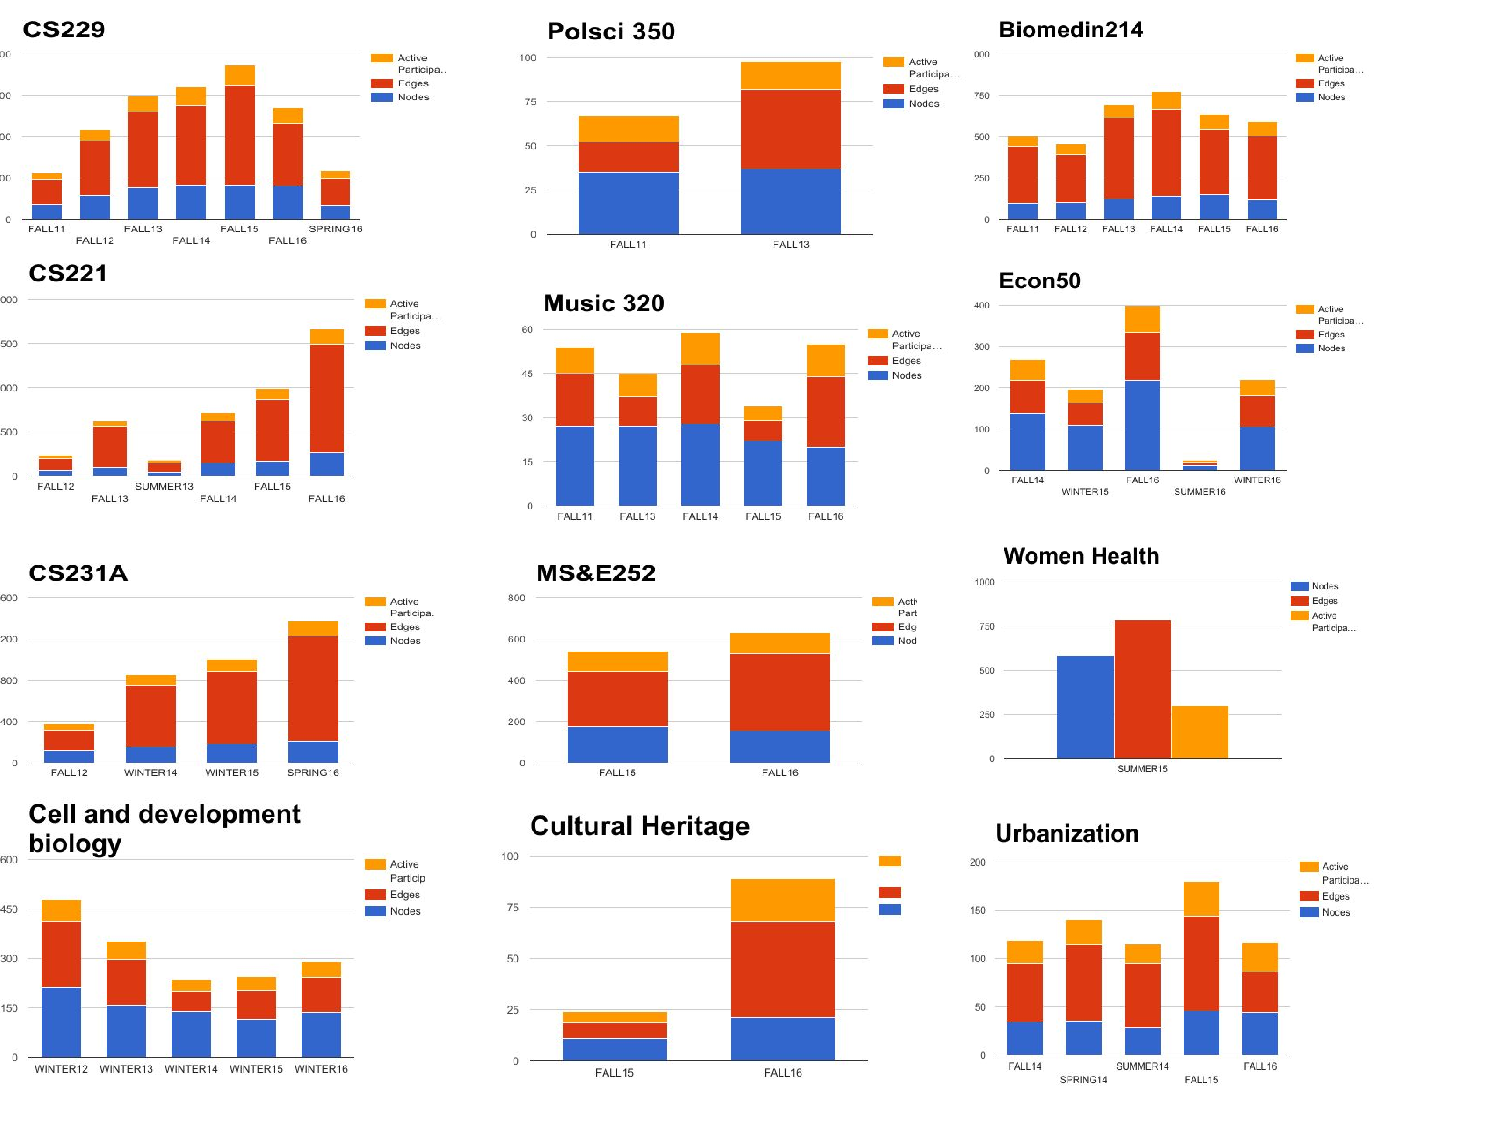
\includegraphics[width=1.2\textwidth]{Figs/nodes2.pdf}
       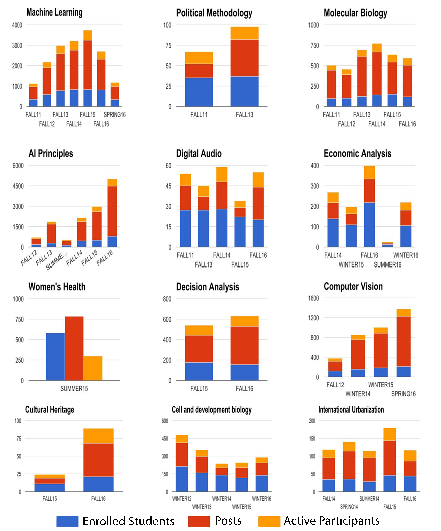
\includegraphics{Figs/classesInDatasetLegendAltered.pdf}
       \caption{\textnormal{Number of students enrolled in the course,
           number of students active in the forum, and number
           postings.}}
       \label{fig:simpleCrsStats}
\end{figure}
 
 
% \begin{table}[]
% \centering
% \caption{Summary of Courses Used for Analysis}
% \label{tab:simpleCrseStats}
% \begin{tabular}{lllll}
% \multicolumn{1}{c}{\textbf{Course}}                                                  & \multicolumn{1}{c}{\textbf{Offering}} & \multicolumn{1}{c}{\textbf{\begin{tabular}[c]{@{}c@{}}Number of\\ students\end{tabular}}} & \multicolumn{1}{c}{\textbf{\begin{tabular}[c]{@{}c@{}}Students\\ with posts\end{tabular}}} & \multicolumn{1}{c}{\textbf{\begin{tabular}[c]{@{}c@{}}Percentage\\ forum participation\end{tabular}}} \\
% \textbf{\begin{tabular}[c]{@{}l@{}}Artificial\\   Intelligence\end{tabular}}         & FALL12                                & 192                                                                                       & 106                                                                                        & 55\%                                                                                                  \\
% \textbf{}                                                                            & FALL13                                & 278                                                                                       & 195                                                                                        & 70\%                                                                                                  \\
% \textbf{}                                                                            & FALL14                                & 435                                                                                       & 291                                                                                        & 67\%                                                                                                  \\
% \textbf{}                                                                            & FALL15                                & 494                                                                                       & 357                                                                                        & 72\%                                                                                                  \\
% \textbf{}                                                                            & FALL16                                & 782                                                                                       & 529                                                                                        & 68\%                                                                                                  \\
% \textbf{}                                                                            & SUMMER13                              & 137                                                                                       & 81                                                                                         & 59\%                                                                                                  \\
% \textbf{Machine Learning}                                                            & FALL11                                & 356                                                                                       & 166                                                                                        & 47\%                                                                                                  \\
% \textbf{}                                                                            & FALL12                                & 581                                                                                       & 283                                                                                        & 49\%                                                                                                  \\
% \textbf{}                                                                            & FALL13                                & 776                                                                                       & 383                                                                                        & 49\%                                                                                                  \\
% \textbf{}                                                                            & FALL14                                & 820                                                                                       & 449                                                                                        & 55\%                                                                                                  \\
% \textbf{}                                                                            & FALL15                                & 827                                                                                       & 489                                                                                        & 59\%                                                                                                  \\
% \textbf{}                                                                            & FALL16                                & 803                                                                                       & 393                                                                                        & 49\%                                                                                                  \\
% \textbf{}                                                                            & SPRING16                              & 331                                                                                       & 189                                                                                        & 57\%                                                                                                  \\
% \textbf{Computer Vision}                                                             & FALL11                                & 59                                                                                        & 29                                                                                         & 49\%                                                                                                  \\
% \textbf{}                                                                            & FALL12                                & 120                                                                                       & 62                                                                                         & 52\%                                                                                                  \\
% \textbf{}                                                                            & SPRING16                              & 208                                                                                       & 150                                                                                        & 72\%                                                                                                  \\
% \textbf{}                                                                            & WINTER14                              & 152                                                                                       & 101                                                                                        & 66\%                                                                                                  \\
% \textbf{}                                                                            & WINTER15                              & 180                                                                                       & 125                                                                                        & 69\%                                                                                                  \\
% \textbf{Decision Analysis}                                                           & FALL15                                & 176                                                                                       & 100                                                                                        & 57\%                                                                                                  \\
% \textbf{}                                                                            & FALL16                                & 156                                                                                       & 104                                                                                        & 67\%                                                                                                  \\
% \textbf{\begin{tabular}[c]{@{}l@{}}Computational Molecular\\   Biology\end{tabular}} & FALL11                                & 96                                                                                        & 61                                                                                         & 64\%                                                                                                  \\
% \textbf{}                                                                            & FALL12                                & 101                                                                                       & 67                                                                                         & 66\%                                                                                                  \\
% \textbf{}                                                                            & FALL13                                & 123                                                                                       & 80                                                                                         & 65\%                                                                                                  \\
% \textbf{}                                                                            & FALL14                                & 140                                                                                       & 103                                                                                        & 74\%                                                                                                  \\
% \textbf{}                                                                            & FALL15                                & 147                                                                                       & 93                                                                                         & 63\%                                                                                                  \\
% \textbf{}                                                                            & FALL16                                & 120                                                                                       & 86                                                                                         & 72\%                                                                                                 
% \end{tabular}
% \end{table}


\begin{figure}[]
       \centering
       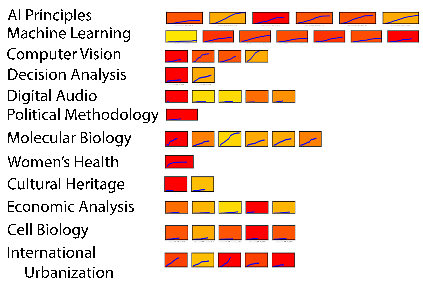
\includegraphics[width=1\textwidth]{Figs/smallMultiplesPostings.pdf}
       \caption{\textnormal{Average postings across a quarter by top
           10\% students in different course offerings. Vertical scale
           is the same for all swatches.
       }}
       \label{fig:smallMults}
\end{figure}

From the forum posts of these data we constructed one social graph for
each course offering. We then analyzed changes in two social graph
measures over time to find `important' weeks.

\section{From Posts to Connection Graph}

Social networks are most simply modeled by considering each
participant as a node, and interactions initiated by participants as
out-directed links. In our case each node represents a student,
i.e. we only define one type of node. Links in our forum interaction
graph represent one student posting, or comment on another student's
contribution. That is, our links are unidirectional. Multiple
interaction initiations by one student are captured by weighting the
corresponding outgoing links. Many graph analysis tools operate on
models of this type.

Other strategies for viewing forum traffic as a graph exist to cover
different goals. For example, \cite{Anwar2013} additionally consider
posts themselves as one type of node. Linkages between the post nodes
represent topics connections. Similarly, when user communication
facilities operate on particular platforms, such as underground
forums, which include private `buddy' connections, then such
facilities may need to be modeled as well \cite{Moto2011}.

For the purpose of identifying candidate time points for encouraging
online conversation participation our chosen model suffices. Note that
this work does not consider additional measures, such as content
quality, for which a richer model would be required.

Many measures are used to quantify various aspects of social graphs
\cite{hann2005, lesk14}. Not all are meaningful in the context of
education-related forum interactions. We focus here on two measures:
{\em weighted out-degree}, and {\em page
  rank}. Figure~\ref{fig:forumGraph} illustrates our use of social
graphs for forum activity.
\begin{figure}[]
       \centering
       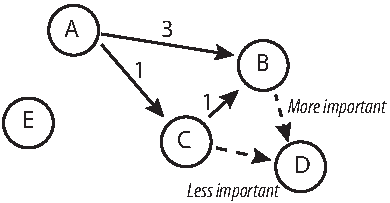
\includegraphics[width=1.0\textwidth]{Figs/forumNetworkExample.pdf}
       \caption{\textnormal{Example social graph induced by forum posts.}}
       \label{fig:forumGraph}
\end{figure}
Nodes $A$, $B$, $C$, $D$, and $E$ represent students. The link from
$A$ to $B$ is marked with the number $3$, because $A$ commented three
times on one or more of $B$'s posts. The number of outgoing links is
the node's {\em out-degree weight}. For example, the {\em out-degree
  weight} of $A$ is $4$.

The number of incoming links is called the node's {\em
  in-degree}. Node $C$'s in-degree is $1$. Node $E$ has no links
entering or exiting. The respective student either did not participate in
the forum or never replied to others posts and never received replies on his posts.

Analogous to Web pages, each node can be assigned a {\em page
  rank}. The intuition in this context is that student $S_1$'s
presence in the forum is more `important' than student $S_2$'s if the
node representing $S_1$ has higher page rank than the node that
represents $S_2$. In our context the intuition behind page rank is
that a node $N$ is more important (has higher page rank) the more
other important nodes comment on $N$'s posts. Imagine a scenario in
which student $S_1$ posts an interesting question, to which many
students comment with their opinion, creating a long thread. The node
representing $S_1$ would experience an increase of its page rank with
every incoming comment. Node $B$ in Figure~\ref{fig:forumGraph} is an
example for this situation. Its in-degree weight is $4$. If $B$ were
to comment on one of $D$'s posts, then $D$'s page rank would increase
more than if the low-page-rank node $C$ commented on $D$.

In terms of evaluating a student's participation in the forum, a high
page rank, and high out-degree are positive. Low values are less
positive. We chose these two values because of their relatively
straight-forward meanings when applied to forum posts, and for their
relevance to our goal of identifying potential intervention times.
%% Figure~\ref{fig:smMultsPageRank} shows a summary of how average page
%% ranks for the top-10\% contributors changes.
%% \begin{figure}[]
%%        \centering
%%        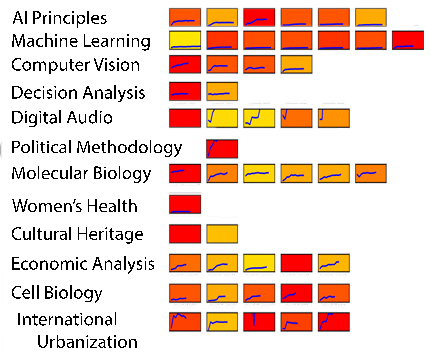
\includegraphics{Figs/smallMultiplesPageRank.pdf}
%%        \caption{\textnormal{Summary of average page rank over top-10\%
%%            of students across successive offerings.}}
%%        \label{fig:smMultsPageRank}
%% \end{figure}
Some of the fifteen other measures we computed, such as {\em
  betweenness} are meaningful for forum scenarios as well, but their
usefulness depends on one's analysis goals. For example,
\cite{yang2013} include several of those measures for the purpose of
persistence prediction. For evaluating contribution {\em quality} the
contents of posts would need to be considered: students who
persistently post irrelevant contents contribute less positively to
the forum than constructively participating students. However, for our
purposes the two measures of page rank and out-degree provide strong
enough signals. We in fact focus in the following material on the
weighted out-degree to explore its contributions to insights into
student behavior.

\section{Analysis Procedure}

For each course we identified the top 10\% students who contributed
the most to the forum. For those students we computed the average of
our chosen social graph measures. This average was computed for each
week of each offering. The results provided a week-by-week time series
of postings and evolving pagerank for these students.

Figure~\ref{fig:cs229OutDeg} shows a typical time series with the sum
of postings (i.e. weighted out degree) on the ordinal, and weeks into
the quarter on the abscissa.
%% \begin{figure}[htp]
%%        \centering
%%        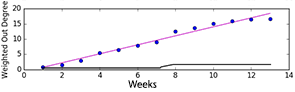
\includegraphics{Figs/comparison_Weighted_Out_Degree_fall16SimplifiedSmall.png}
%%        \caption{\textnormal{Forum post contributions by top 10\% of
%%            contributors throughout an academic quarter (machine learning class).}}
%%        \label{fig:cs229OutDeg}
%% \end{figure}
\begin{figure}[]
       \centering
       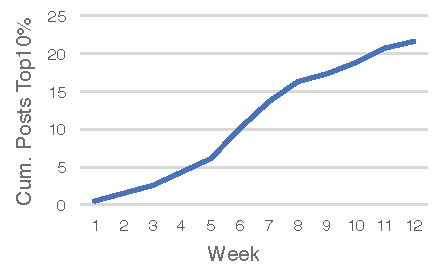
\includegraphics{Figs/CS229Fall15DataContributionsNoFrills.pdf}
       \caption{\textnormal{Cumulative number of postings by the top 10\% of
           contributors throughout an academic quarter (machine
           learning class).}}
       \label{fig:cs229OutDeg}
\end{figure}
Notice in Figure~\ref{fig:cs229OutDeg} that the successive increases
in average contribution of the top 10\% appear to take a jump after
week 5. Such a discontinuity, or {\em change point} could be a good
trigger for encouraging students who have held back participation. For
example, the jump could be due to important discussions just before
the midterm.

However, visual inspection is insufficient for determining whether
this change is statistically significant, or could instead be
explained by random noise. The question mark in the figure is a
reminder of this uncertainty.

Therefore, we next performed an analysis aimed at quantifying how much
a given increase or decrease in weekly posts differed from the mean of
those variations. For each series of course offerings this analysis
yielded insight into how consistent the location of change points was
across multiple offerings of the same course. Such consistency across
offerings would imply that an instructor could `hard code' the week(s)
in which encouragements would be sent.

From an offering's weekly count of total posts to date by the top 10\%
contributors, we constructed the incremental increase of posts for each
week. For example, Figure~\ref{fig:cs229ChangePts}'s top line shows
the incremental contributions for each week of the same machine
learning offering shown in Figure~\ref{fig:cs229OutDeg}

In order to discover for each week whether its number of contributions
differed significantly from those of other weeks, we performed a
bootstrap procedure across the post-contribution increments, i.e. over
the data points of the top line in Figure~\ref{fig:cs229ChangePts}
\cite{tayl16}
\begin{figure}[]
       \centering
       \includegraphics{Figs/cs229Fall15_changePointFinalStyledPlusRawData.pdf}
       \caption{\textnormal{Change points in forum posting 
           time series of a machine learning course.}}
       \label{fig:cs229ChangePts}
\end{figure}
This process takes as reference the {\em CUSUM} (cumulative sum) over the incremental
post counts \cite{nist2012}. This quantity is computed for each week
as the sum of differences from the overall mean of incremental posts.
\begin{equation}
S_m = \sum_{i=0}^{m}(x_i-\hat{\mu}_0)
\end{equation}
where $x_i$ is the $i$'th weekly post increment, and $\hat{\mu}_0$ is
the mean across all the weekly post increments.

Our bootstrap permuted the post increments, and re-computed the CUSUM
points 1000 times. For each permutation we computed the $S_{diff}^0 =
S_{max}^0-S_{min}^0$ of the resulting CUSUM, and determined whether
$S_{diff}^0$ was less than the corresponding value $S_{diff}$ in the
CUSUM of the correctly ordered number of posts. $S_{max}^0$ and
$S_{min}^0$ are the maximum/minimum values of the CUSUM for a given
iteration. Their difference represents the farthest that the
iteration's CUSUM strays from the CUSUM's mean.

We compute a confidence $C$ that a change point occurred sometime in a
quarter via:
\begin{equation}
  \begin{split}
    x_i = \left.
    \begin{cases}
      1, & \mbox{for } S_{diff}^0 < S_{diff} \\
      0, & \mbox{for }S_{diff}^0 >= S_{diff}
    \end{cases}
    \right.
  \end{split}
\end{equation}
\begin{equation}
  \label{eqn:confidence}
  C = \left.
  100*\frac{\sum_1^N x_i}{N}
  \right.
\end{equation}
where $x_i$ is the outcome of one bootstrap iteration, and $N$ is the
number of bootstrap iterations. Figure~\ref{fig:multiBoots} shows an
example of five iterations. Points on the unlabeled lines denote
differences of CUSUM points from the mean during one week. Note that
the distance of those lines from the dotted mean line tends to be
much smaller than the CUSUM distance for the correctly sequenced
values at the bottom.
\begin{figure}[]
       \centering
       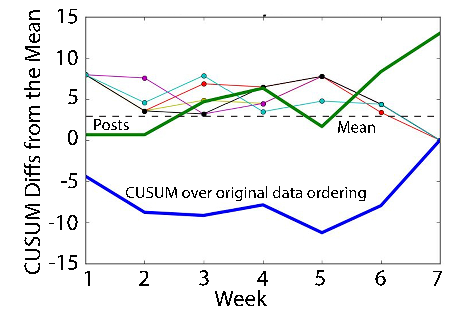
\includegraphics{Figs/multiBootstrapCurvesUrbStud145Summer14.pdf}
       \caption{\textnormal{CUSUMs from permuted weekly post
           contribution rates hover around the mean.}}
       \label{fig:multiBoots}
\end{figure}
Following \cite{tayl16} we determined the last week before a change
for each change point. Figure~\ref{fig:cs229ChangePts} shows an
example.

The bottom chart's line shows again the weekly post contributions.
Up to about week four, weekly postings by the top-10\% was below
average. The corresponding downward segment of the CUSUM reflects
increasingly negative sums of those differences. During week 5 weekly
contributions begin to rise above the mean, and the CUSUM `recovers'
upward towards zero.

The horizontal (red) lines in the top chart indicate the upper and
lower limits within which week-to-week differences in posts
contributions would be expected to vary just by
chance\footnote{Assuming normal distribution of contribution
  difference values}. The lines are called {\em control limits}, and
we will discuss their potential real-time use during a course's run
time in Section~\ref{sec:discussion}.

The vertical bands in Figure~\ref{fig:cs229ChangePts} (bottom)
indicate visually where a significant change in contribution rate
occurred. In this case the sharp increase at week five was found via
Equation~\ref{eqn:confidence} to be a true change point at confidence
level 92\%.

\section{Results and Discussion}
\label{sec:discussion}

Our question was ``when would be good times during a course for
encouraging students who lag behind in forum contributions?'' We
hypothesize that times when the top 10\% of contributors speed up,
other students might be encouraged to do the same.

Table~\ref{tbl:consistency} shows the weeks in which different courses
tended to experience significant changes in behaviors of the top-10\%
contributors. The percentages in a week's column indicate the
proportion of the respective course's offerings that experienced jumps
during that week.
\begin{table*}[htbp]
\centering
\caption{Consistency across offerings in weeks with change points.}
\label{tbl:consistency}
\begin{tabular}{lcccccccc}
Course                                                                                           & \multicolumn{1}{l}{Week3} & \multicolumn{1}{l}{Week4} & \multicolumn{1}{l}{Week5} & \multicolumn{1}{l}{Week6} & \multicolumn{1}{l}{Week7} & \multicolumn{1}{l}{Week8} & \multicolumn{1}{l}{Week9} & \multicolumn{1}{l}{Week10} \\ \cline{2-9} 
\multicolumn{1}{l|}{AI Principles}                                                               & \multicolumn{1}{c|}{17\%} & \multicolumn{1}{c|}{}     & \multicolumn{1}{c|}{}     & \multicolumn{1}{c|}{}     & \multicolumn{1}{c|}{50\%} & \multicolumn{1}{c|}{16\%} & \multicolumn{1}{c|}{33\%} & \multicolumn{1}{c|}{}      \\ \cline{2-9} 
\multicolumn{1}{l|}{Machine Learning}                                                            & \multicolumn{1}{c|}{50\%} & \multicolumn{1}{c|}{}     & \multicolumn{1}{c|}{14\%} & \multicolumn{1}{c|}{14\%} & \multicolumn{1}{c|}{14\%} & \multicolumn{1}{c|}{28\%} & \multicolumn{1}{c|}{}     & \multicolumn{1}{c|}{}      \\ \cline{2-9} 
\multicolumn{1}{l|}{Computer Vision}                                                             & \multicolumn{1}{c|}{}     & \multicolumn{1}{c|}{}     & \multicolumn{1}{c|}{}     & \multicolumn{1}{c|}{50\%} & \multicolumn{1}{c|}{}     & \multicolumn{1}{c|}{}     & \multicolumn{1}{c|}{}     & \multicolumn{1}{c|}{}      \\ \cline{2-9} 
\multicolumn{1}{l|}{Decision Analysis}                                                           & \multicolumn{1}{c|}{50\%} & \multicolumn{1}{c|}{50\%} & \multicolumn{1}{c|}{50\%} & \multicolumn{1}{c|}{}     & \multicolumn{1}{c|}{}     & \multicolumn{1}{c|}{50\%} & \multicolumn{1}{c|}{}     & \multicolumn{1}{c|}{}      \\ \cline{2-9} 
\multicolumn{1}{l|}{\begin{tabular}[c]{@{}l@{}}Algorithms for \\ Molecular Biology\end{tabular}} & \multicolumn{1}{c|}{}     & \multicolumn{1}{c|}{}     & \multicolumn{1}{c|}{}     & \multicolumn{1}{c|}{}     & \multicolumn{1}{c|}{33\%} & \multicolumn{1}{c|}{}     & \multicolumn{1}{c|}{}     & \multicolumn{1}{c|}{}      \\ \cline{2-9} 
\multicolumn{1}{l|}{\begin{tabular}[c]{@{}l@{}}International \\ Urbanization\end{tabular}}       & \multicolumn{1}{c|}{}     & \multicolumn{1}{c|}{}     & \multicolumn{1}{c|}{}     & \multicolumn{1}{c|}{20\%} & \multicolumn{1}{c|}{}     & \multicolumn{1}{c|}{}     & \multicolumn{1}{c|}{}     & \multicolumn{1}{c|}{}      \\ \cline{2-9} 
\end{tabular}
\end{table*}
The results indicate that week six is particularly likely to
experience changes in posting rates. We can hypothesize that the
traffic is related to midterms. Week eight might be related to final
projects coming due not too far out.

Except for the urban studies course the only courses with regularities
of change points among their offerings are science and engineering
courses. The humanities and social sciences, while using forum
facilities, have not included the forum as a central discussion
hub. The numbers of students attending these courses are also
smaller than the science/engineering classes.

When computing the percentages of Table~\ref{tbl:consistency} we
included all offerings, reaching back to 2011. This year was one of
the earliest that Piazza offered forum services. It is possible that
as forum use continues to gain momentum, more regular patterns might
emerge.

The forum change point computations we outlined above require data
from all weeks of an offering to be available. In the presence of
historic data this requirement is not a problem. But what could an
instructor do to discover unusual posting frequencies while the
offering is running?

\subsection{Control Charts for Forum Alerts}
Figure~\ref{fig:cs229ChangePts}'s lower chart hints at a possibility we
have not yet discussed. As mentioned, the horizontal dotted lines are
{\em process limits}, a term from process control practice
\cite{nist2012}. The limits bound the values within which a process is
expected to vary. For industrial processes the variations might lie
around a known optimal operating level, such as a temperature. When no
such level is known from the domain, a mean can be used.

In the context of instructional forum use it would be possible to
detect points, such as the one above the upper control limit in
Figure~\ref{fig:cs229ChangePts}. Such change to above-normal might
indicate confusion among the students, or the discovery of an exciting
topic. Either way, the instructor's attention might be warranted, as
might be pointing passive students to the increased activity.

\subsection{Personalized, Quantitative Encouragement}
The data framework we discussed could also be deployed to provide
personalized encouragement for passive students. Rather than
admonishing students for past passivity, a forward-looking nudge could
be provided. Figure~\ref{fig:nudgeAngles} illustrates this option.
\begin{figure}[]
       \centering
       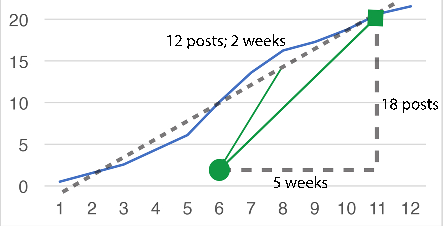
\includegraphics{Figs/angleTrajectories.pdf}
       \caption{\textnormal{Personalized, quantitative nudges:
           catching up with the top-10\% within five weeks, or two
           weeks.}}
       \label{fig:nudgeAngles}
\end{figure}
The dot represents one student and their contribution as of week six:
two postings. Two of many possible options are shown in the Figure for
catching up to the top-10\% contributors. These, and other options are
derived by drawing a line from the student's position to an
intersection with the regression line. That line is known from past
course offerings. The larger the slope of the connecting line, the
more aggressive the plan for catching up. For example, the long line
would catch the student up within five weeks, assuming a weekly rate
of $(20-2)/5 \approx 4$ messages per week.

Alternatively, the shorter line would call for six messages per week,
to catch up within two weeks. The square at the end of the long option
is intended to represent a slider that the student could run along the
regression line to make a plan. The number of required weekly messages
would be updated continuously as the student operates the
slider. While this sketch is certainly not the ideal, and ultimate
user interface, it illustrates the ideas of using past and current
forum data to provide ({\em i}) forward-looking encouragement in place
of recrimination, and ({\em ii}) to empower the student by
personalizing the message, and providing a tool for planning.


Yeomans et al. \cite{Yeomans} suggest that planning prompts can help
learners adopt productive frames of mind at the outset of a learning
goal that encourage and forecast student success. They hypothesize
that prompting MOOC students to plan their efforts at the start of a
course will increase completion rates.

There have been many studies on the factors determining the decline
rate in forum participation \cite{DBLP}, and student dropout rates
\cite{Yang_peerinfluence} with the progression of courses in MOOC
contexts. Anderson et al. \cite{DBLP:journals/corr/AndersonHKL14}
examine the behavioral patterns of high- and low-achieving students
and relate student's final grade to their engagement in MOOCS.

\section{Conclusion and Future Work}

We studied how forum posting rates vary week to week across about 40
offerings of courses. We included science, engineering, music,
political science, urban studies courses, and others. The purpose was
an investigation whether particular weeks in each quarter often stand
out as featuring significant changes in post rates. We found that such
weeks exist, albeit not with perfect consistency, and mostly limited
to science and engineering courses. We also sketched a method for
personalizing encouragement messaging. The effectiveness of this
approach is unproven, and is the subject of further study.

The important next step is to test whether encouragements at the
change points are in fact more effective than encouragement offered,
for example, at the beginning of a course. Equally important is to
extend our study to include measures of post quality. We focused on
the top 10\% most prolific forum contributors. But the quality of
those postings---by some measure---is important to include in
evaluations of forum health. For that exploration we will include both
page content and the page ranks we computed for this work.  Our graph
based approach has generated the necessary framework for this future
investigation.

A further use of page rank will be the ability to observe how teaching
assistants interact with students around particular topics. TAs will
tend to have high page rank, and by filtering page rank computations
by the topics of student postings we can expect to see topic-based
divisions of labor among the assistants. They can then more formally
distribute their load.

Forum facilities offer potential for student interaction outside the
classroom. One hopes that courses with a large component of discussion
might benefit in the future. Meanwhile, it is important to develop
methods that help all students take advantage of these online contact
options. This work is a step in that direction.

%% Control charts are of significance for our scenario, because
%% breakages across control bounds can be observed at any point in
%% time. Instructors could therefore be alerted weekly of any students
%% (or average of larger student groups) who are atypical in their
%% posting behavior. Bootstrap procedures, which permute data points many
%% times, computing target measures like means each time require that all
%% data points are available for the procedure. On the other hand, these
%% procedures can detect multiple change points that occur in the
%% examined data.



%% Figure~\ref{fig:smOutDeg} shows a summary of these series for some of
%% the course offerings. We provide more detailed views further on.
%% \begin{figure}[htp]
%%        \centering
%%        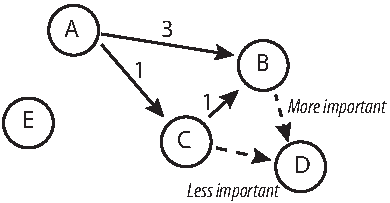
\includegraphics[width=1.0\textwidth]{Figs/forumNetworkExample.pdf}
%%        \caption{\textnormal{Example social graph induced by forum posts.}}
%%        \label{fig:smOutDeg}
%% \end{figure}

%% \begin{table*}[t]
%% \centering
%% \resizebox{\columnwidth}{!}{%
%% \caption{Summary of Examined Courses}
%% \label{tab:courseStats}
%% \begin{tabular}{@{}|>{\columncolor[gray]{0.92}}c|c|c|c|c|c|c|c|c|c|@{}}
%% \hline
%% \rowcolor{green!25}
%% \textbf{Course} & \textbf{Offering} & \textbf{Nodes} & \textbf{Edges}  & \textbf{Contributions}  & \textbf{Density} & \textbf{Active Participants} & \textbf{Largest SCC} & \textbf{Largest WCC} \\ \hline
%% \textbf{Artificial Intelligence}  & FALL12            & 192            & 414                                & 893  &0.011289267015706806                                            & 106                          & 52                                                    & 105                                                 \\ \hline
%%                 & FALL13            & 278            & 1396           & 4629 &0.018128457522790433                                                                     & 195                          & 130                                                   & 194                                                 \\\hline
%%                 & FALL14            & 435            & 1423                                   & 4352 &0.007537475501880396                                              & 291                          & 149                                                   & 290                                                 \\  \hline
%%                 & FALL15            & 494            & 2114           & 4220 &0.008680227640406993                                         & 357                          & 197                                                   & 352                                                 \\ \hline
%%                 & FALL16            & 782            & 3699           & 7286                                 &0.006056567257532641 &529                          & 332                                                   & 529                                                  \\ \hline
%%                 & SUMMER13          & 137            & 320            & 917 &0.017174753112924                       & 81                           & 39                                                    & 76                                                  \\ \hline 
%% \textbf{Machine Learning} & FALL11   & 356   & 601   & 1237                          & 0.004755499287862003  & 166                 & 60                                           & 164                                        \\ \hline
%%                & FALL12   & 581   & 1306  & 2663                        & 0.0038756009258709718 & 283                 & 120                                          & 282                                        \\ \hline
%%                & FALL13   & 776   & 1823  & 4649                       & 0.003031260392417692  & 383                 & 158                                          & 375                                        \\ \hline
%%                & FALL14   & 820   & 1943  & 3610                       & 0.002893177283421186  & 449                 & 168                                          & 446                                        \\ \hline
%%                & FALL15   & 827   & 2413  & 5553                          & 0.0035324153640305545 & 489                 & 219                                          & 489                                        \\ \hline
%%                & FALL16   & 803   & 1510  & 3140                           & 0.002344698651875914  & 393                 & 153                                          & 386                                        \\ \hline
%%                & SPRING16 & 331   & 657   & 1548                           & 0.006014831090359792  & 189                 & 65                                           & 
%%                187      \\ \hline
%% \textbf{Computer Vision} & FALL11   & 59    & 84    & 248                             & 0.024547048509643482 & 29                  & 12                                           & 29                                         \\ \hline
%%        & FALL12   & 120   & 195   & 528                            & 0.01365546218487395  & 62                  & 16                                           & 62                                         \\ \hline
%%        & SPRING16 & 208   & 1018  & 3722                           & 0.023643626904496468 & 150                 & 93                                           & 150                                        \\ \hline
%%        & WINTER14 & 152   & 601   & 1618                           & 0.026185081910073196 & 101                 & 63                                           & 100                                        \\ \hline
%%        & WINTER15 & 180   & 702   & 1639                           & 0.021787709497206705 & 125                 & 87                                           & 125                                                                        \\ \hline
%% \textbf{Decision Analysis} 
                
%%                   & FALL15   & 176   & 265   & 445                           & 0.008603896103896103 & 100                 & 10                                           & 95                                         \\ \hline
%%                   & FALL16   & 156   & 373   & 1185                          & 0.015425971877584781 & 104                 & 44                                           & 104  \\ \hline                                     
%% \textbf{Computational Molecular Biology} & FALL11   & 96    & 348   & 653                            & 0.038157894736842106 & 61                  & 38                                           & 61                                         \\ \hline
%%                   & FALL12   & 101   & 289   & 657                           & 0.028613861386138615 & 67                  & 41                                           & 67                                         \\ \hline
%%                   & FALL13   & 123   & 490   & 1279                          & 0.03265360522457684  & 80                  & 52                                           & 80                                         \\ \hline
%%                   & FALL14   & 140   & 527   & 1122                          & 0.02708119218910586  & 103                 & 66                                           & 103                                        \\ \hline
%%                   & FALL15   & 147   & 396   & 797                           & 0.018451216102879506 & 93                  & 45                                           & 92                                         \\ \hline
%%                   & FALL16   & 120   & 384   & 886                           & 0.02689075630252101  & 86                  & 54                                           & 86       \\                                 
%% \hline

%% \textbf{International Urbanization Seminar} & FALL14   & 34    & 61    & 419                             & 0.054367201426024955 & 23                  & 9                                            & 23                                         \\ \hline
%%                     & SPRING14 & 35    & 79    & 379                           & 0.06638655462184874  & 26                  & 8                                            & 26                                         \\ \hline
%%                     & SUMMER14 & 28    & 67    & 224                             & 0.08862433862433862  & 20                  & 6                                            & 20                                         \\ \hline
%%                     & FALL15   & 46    & 98    & 352                            & 0.04734299516908213  & 36                  & 19                                           & 36                                         \\ \hline
%%                     & FALL16   & 44    & 42    & 165                           & 0.022198731501057084 & 31                  & 4                                            & 31                                         \\ \hline
%% \textbf{Cell and Developmental Biology} & WINTER12 & 214   & 200   & 535                           & 0.004387696897898293  & 65                  & 9                                            & 65                                         \\ \hline
%%                   & WINTER13 & 157   & 140   & 356                           & 0.0057161522129675    & 55                  & 6                                            & 55                                         \\ \hline
%%                   & WINTER14 & 140   & 61    & 85                            & 0.0031346351490236382 & 37                  & 1                                            & 35                                         \\ \hline
%%                   & WINTER15 & 117   & 86    & 135                           & 0.006336575302092543  & 43                  & 5                                            & 43                                         \\ \hline
%%                   & WINTER16 & 136   & 105   & 297                           & 0.005718954248366013  & 49                  & 3                                            & 49                                         \\ \hline
%% \textbf{Economic Analysis} & FALL14   & 138   & 80    & 185                            & 0.004231460911879826  & 50                  & 4                                            & 50                                         \\ \hline
%%                 & WINTER15 & 109   & 54    & 142                        & 0.0045871559633027525 & 33                  & 2                                            & 33                                         \\ \hline
%%                 & FALL16   & 217   & 116   & 460                         & 0.002474825055470217  & 65                  & 10                                           & 65                                         \\ \hline
%%                 & SUMMER16 & 12    & 8     & 21                         & 0.06060606060606061   & 5                   & 2                                            & 4                                          \\ \hline
%%                 & WINTER16 & 106   & 74    & 259                         & 0.006648697214734951  & 39                  & 12                                           & 38                                         \\ \hline
%% \textbf{Indigenous Cultural Heritage} & FALL15   & 11    & 8     & 29                               & 0.07272727272727272 & 5                   & 1                                            & 5                                          \\ \hline
%%                            & FALL16   & 21    & 47    & 62                              & 0.11190476190476191 & 21                  & 5                                            & 20                                         \\ \hline
%% \end{tabular}

%% }
%% \end{table*}

%% \begin{figure}[htp]
%%        \centering
%%        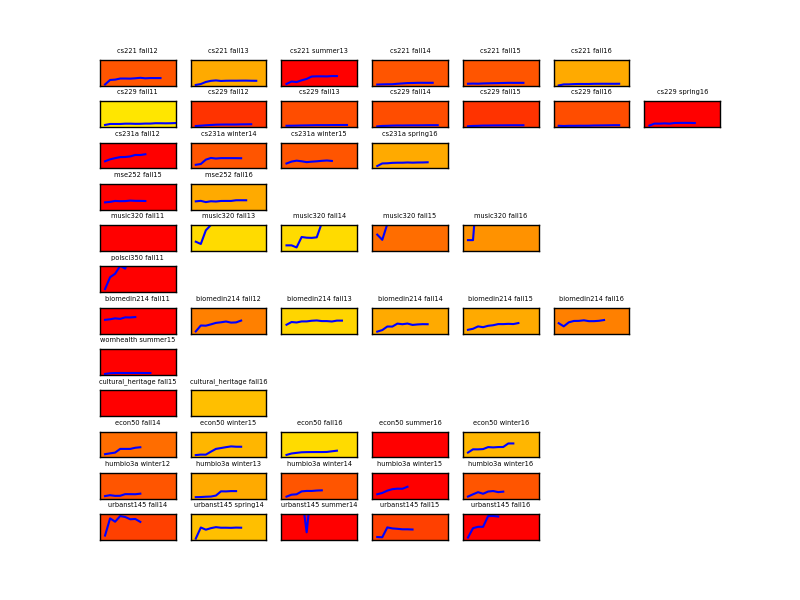
\includegraphics[width=1\textwidth]{Figs/pagerank_sm_color.png}
%%        \caption{\textnormal{Comparison of Pageranks for top 10\% students}}
%%        \label{fig:pageRankCompare}
%% \end{figure}

%% \begin{figure}[htp]
%%        \centering
%%        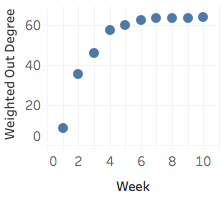
\includegraphics[width=1\textwidth]{Figs/women_health_summer2015_top10.png}
%%        \caption{\textnormal{A MOOC forum post comparison: Women's
%%            Global Health.}}
%%        \label{fig:womenHealth}
%% \end{figure}



